%%git, nb commit, ligne de code, release, j/homme,...
\section{Git}
Nous avons utilisé Git dès le début du projet. Comme nous l'avions presque tous déja utilisé, son utilisation était évidente, sachant qu'en plus, c'est l'un des gestionnaire de code le plus performant.
Nous avons installé un depôt sur le Git du Sif. Nous avons utilisé une branche Master, qui devait contenir uniquement du code compilable, et après, chaque fonctionnalités à été développé sur une branche différentes.
Nous utilisons également Gitg, pour avoir une meilleure vue de l'état de notre dêpot. Voir ~\ref{Gitg} page~\pageref{Gitg}.
\begin{figure}[h]
\caption{\label{Gitg} Capture de Gitg}
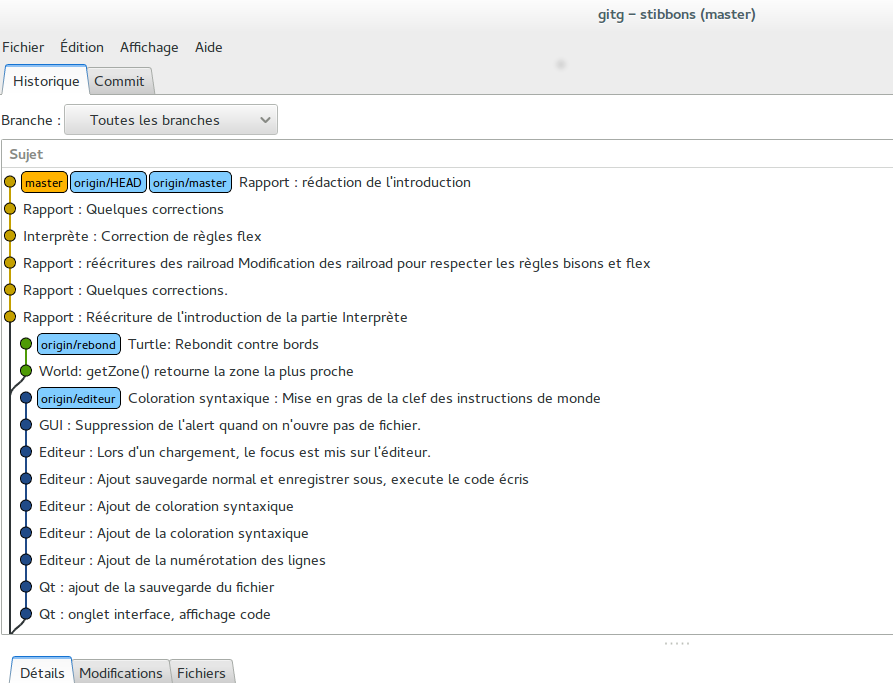
\includegraphics[scale=0.35]{doc/report/gitbranche.png}
\end{figure}


\section{Réalisation}
D'après le backlog final nous avons passé 372 h sur le code, ce qui équivaut, pour 4 personnes, à 93h par personnes, soit environ 13,5 j/homme.
Nous pouvons ainsi estimé un total d'environ 400h pour 4 pour le projet entier (réunions comprises), soit 14,5 j/homme.
L'UE TER M1 est prévu pour 50h par personne (soit 200h pour 4), nous voyons donc que ce quota a été doublé, ce qui n'est pas étonnant.
